\documentclass{standalone}

\begin{document}
\chapter{Results}

The proposed pipeline was developed and applied on the data set described in Chapter \ref{chap:materials}.
The main method for the evaluation of the pre-processing pipeline, i.e. the skull stripping and the tissue segmentation, was a quantitative comparison with the results obtained using the software \textit{FSL} \cite{ART:FSL}, which is a library of functions developed specifically for the analysis of the MRI brain images that became a standard in literature for MR analysis during the last couple of decades \cite{ART:FSL}.
The post-processing pipeline instead was evaluated comparing quantitatively the labels with the manual segmentation of the SCIs provided.

\section{Pre-Processing}
The \textii{FMRIB Software Library (FSL)} became a standard for the analysis of MRI images and then it was decided to use the brain mask obtained with the \textit{BET} function and the segmentation masks (one for each tissue class) obtained using the \textit{FAST} function to use as references for the pre-processing tools developed during this work of thesis.
Another aspect of the proposed pipeline during its development was the execution time that had to be reasonably low in order to give the possibility to use the implemented algorithms also on personal computers.

\subsection{Timing}
One of the main researched feature for the implemented pipeline was the short execution time required to obtain a full segmentation.
It was therefore pre-processed the full data set of $57$ patients, calculating the computation time for each volume. 
Nevertheless the computation time depends on the input size and, as it was shown in the previous chapter, the data set is highly heterogeneous. Since the main difference between images is the size and the spacing on the z-axis, the time results are plotted as a function of the number of slices (i.e. images in planes perpendicular to the z-axis) as it is possible to see in Figure \ref{fig:time_pre}. To obtain the provided data the whole pre-proessing pipeline was performed $8$ times on the entire data set. Of the analysed images $44$ have 30 slices or less and for those images the mean execution times was smaller than 1 minute, $10$ images have a number of slices between $224$ and $288$ and for those images the execution time ranged from $178 \ s$ to $216 \ s$. For the remaining three images with $512$ slices the computation time was about $6 \ min$.

\begin{figure}[h!]
    \centering
    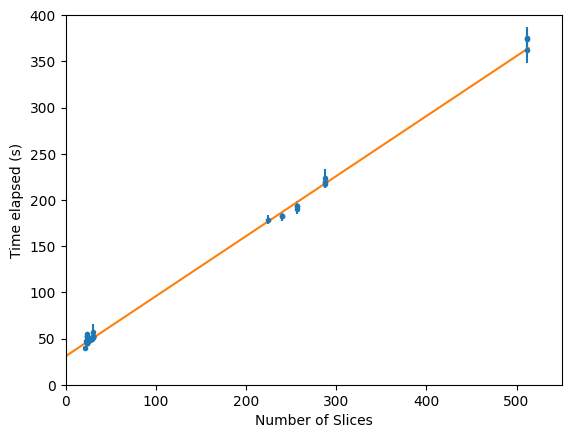
\includegraphics[scale = 0.9]{img/Chap3/times.png}
    \caption{In the Figure is plotted the execution time in function of the number of slices that composed the image. It is possible to see how the execution time increases linearly with the number of slices. In general, for images with 30 slices or fewer the execution time was less than a minute. The maximum values were reached for the images that have 512 slices and is of about $375 \ s$.}
    \label{fig:time_pre}
\end{figure}

The results plotted are obtained running the pipeline on one of the server of the Department of Physics and Astronomy of the University of Bologna, a computer with $32$ CPUs and $126Gb$ of RAM.

%TODO fare il test anche con un piccolo set di immagini sul pc personale.

\subsection{Segmentation Performances}

This sections describes the comparison between the presented pre-processing pipeline and the segmentation obtained using FSL. The comparison was carried out using the dice coefficient presented in equation \ref{eq:Dice}. As described before, this metric provides an overlapping measure; it's range is in [0, 1] where 0 means no overlapping and 1 a perfect overlapping of two binary  volumes.
To provide that measure was chosen to compare the obtained masks (brain mask, white matter, grey matter and cerebrospinal fluid) with the ones obtained with FSL.
The comparison was done on a subset of $56$ over the total data set of $57$ patients. This was because one of the volumes has a incredibly poor resolution the FSL FAST software totally fails in its segmentation.

\paragraph{Brain Extraction:} 
The first process evaluated was the brain extraction. It was measured calculating the Dice coefficient of the overlapping between the brain masks obtained with the proposed pipeline and the ones obtained with the FSL BET function. 
The obtained DSC ranges from a minimum value of $0.47$ to a maximum of $0.96$. As visible in Table \ref{tab:segmentation_metrics}, the mean DSC was $0.87 \pm 0.12$ where the error was evaluated as the standard deviation of the analysed volumes.
The median value for the DSC was $0.93$.


To have a better comprehension of the obtained Dice coefficient values is however necessary to do also a qualitative evaluation of the goodness of the results of FSL. In Figure \ref{fig:FSL_brain} are reported the results of brains extracted with both FSL and the proposed pipeline for a volume which the two software are in agreement leading to a high value for the Dice coefficient, and for a volume in which the FSL BET segmentation partially fails while the proposed pipeline manage in a good segmentation, leading to a low value for the measured metric.
It is therefore necessary to underline that the FSL function result can be optimized by manually change the extraction parameters while the goal researched for the proposed pipeline was to work fully automatically.

\begin{figure}[h!]
		\centering
        \begin{subfigure}[b]{0.325\textwidth}
             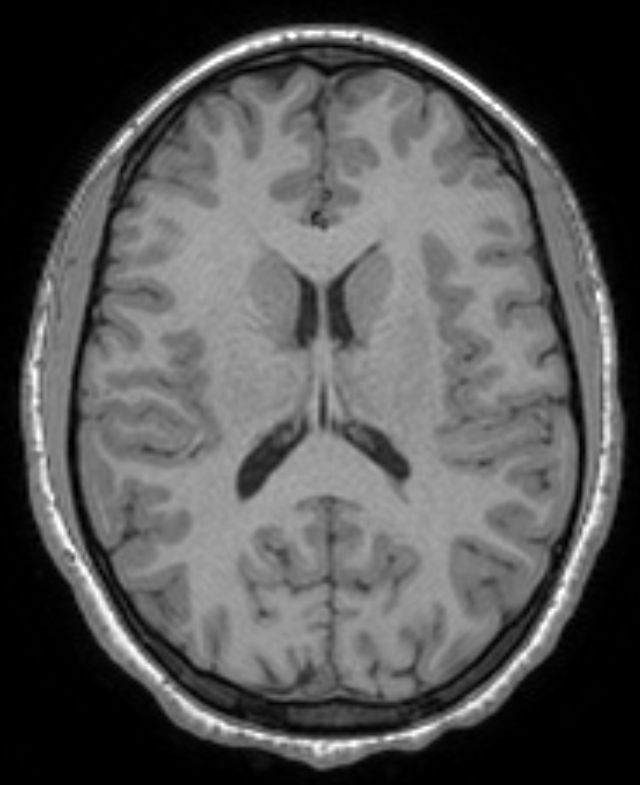
\includegraphics[scale=0.215]{img/Chap3/T1W16.png}
             \caption{Original scan}
        \end{subfigure}
        \hfill
        \begin{subfigure}[b]{0.325\textwidth}
             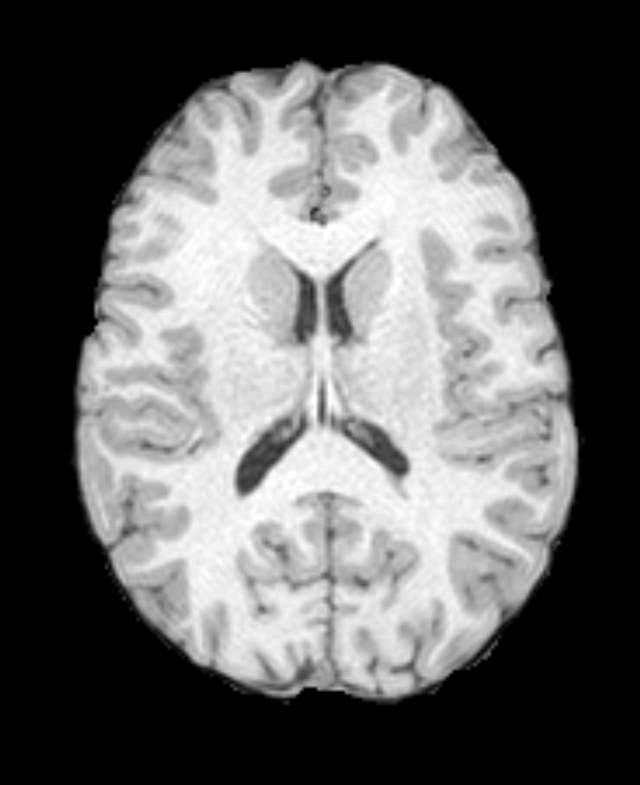
\includegraphics[scale=0.215]{img/Chap3/FSL16.png}
             \caption{Brain extracted with FSL}
        \end{subfigure}
        \hfill
        \begin{subfigure}[b]{0.325\textwidth}
             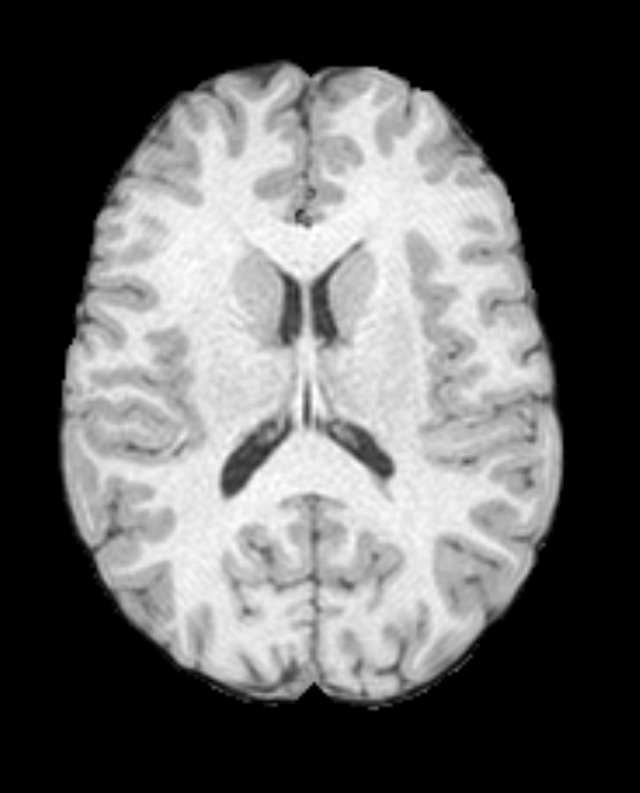
\includegraphics[scale=0.213]{img/Chap3/BRAIN16.png}
             \caption{Implemented pipeline}
        \end{subfigure}
        \hfill
        \begin{subfigure}[b]{0.325\textwidth}
             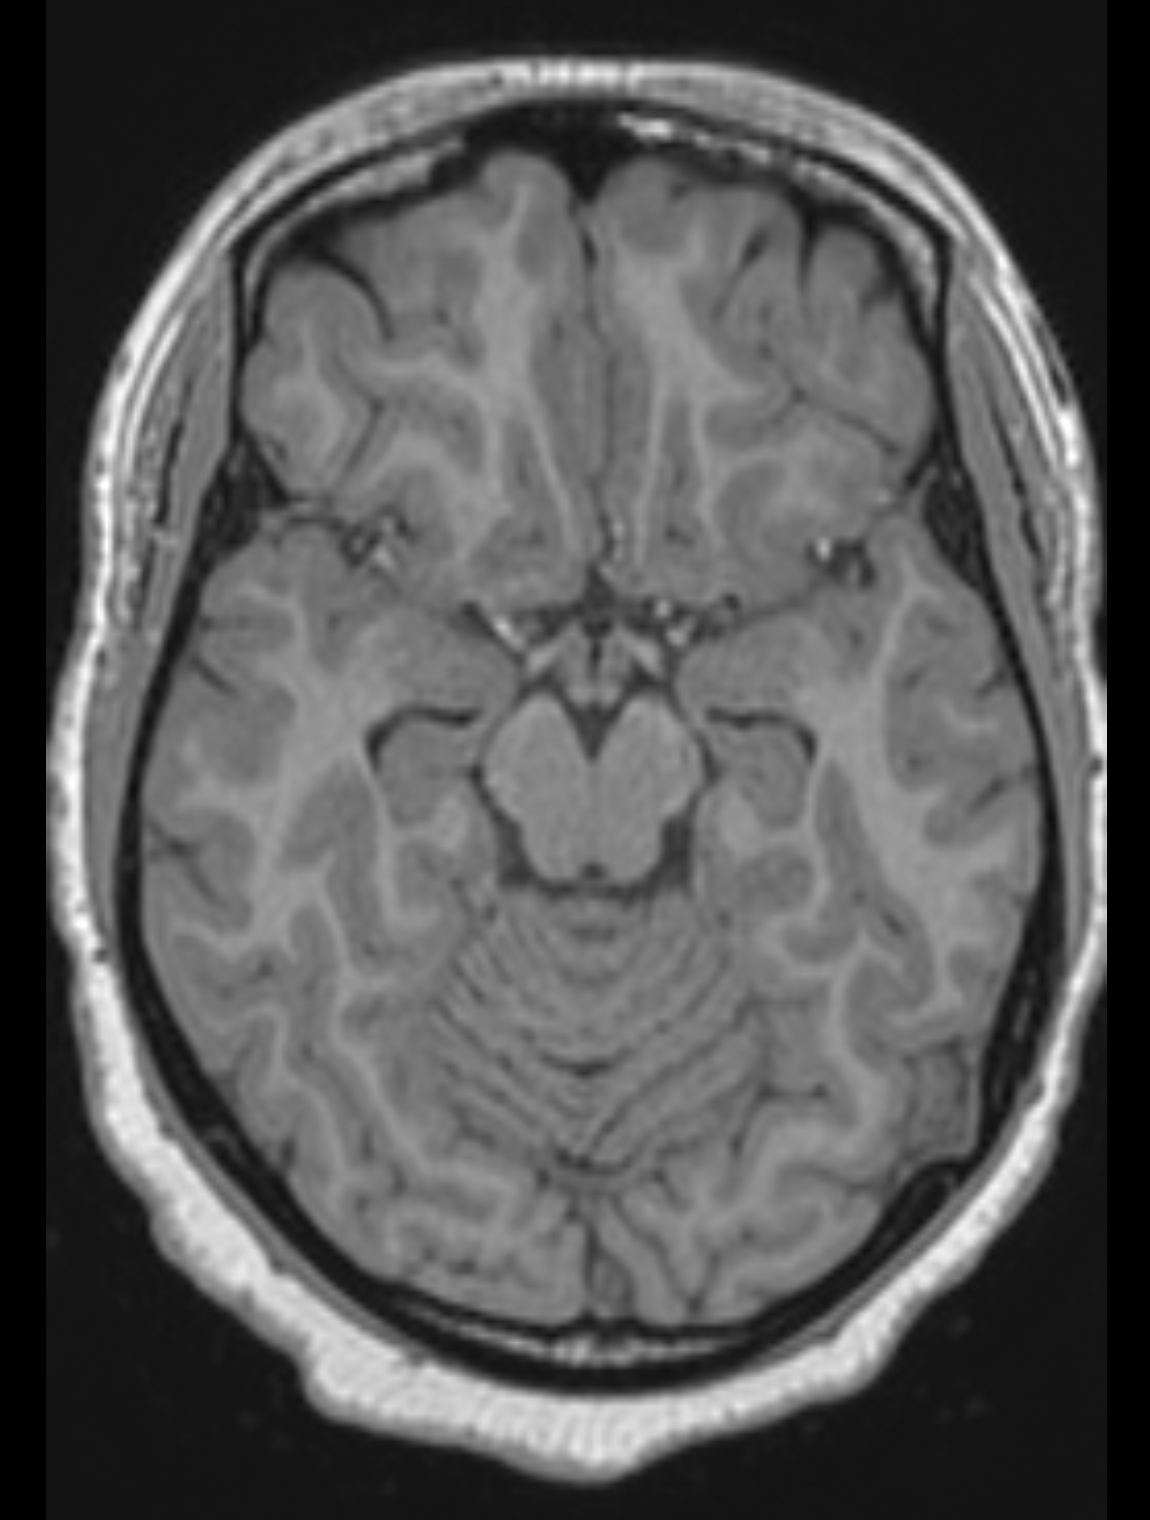
\includegraphics[scale=0.12]{img/Chap3/T1W54.jpg}
             \caption{Original scan}
        \end{subfigure}
        \hfill
        \begin{subfigure}[b]{0.325\textwidth}
             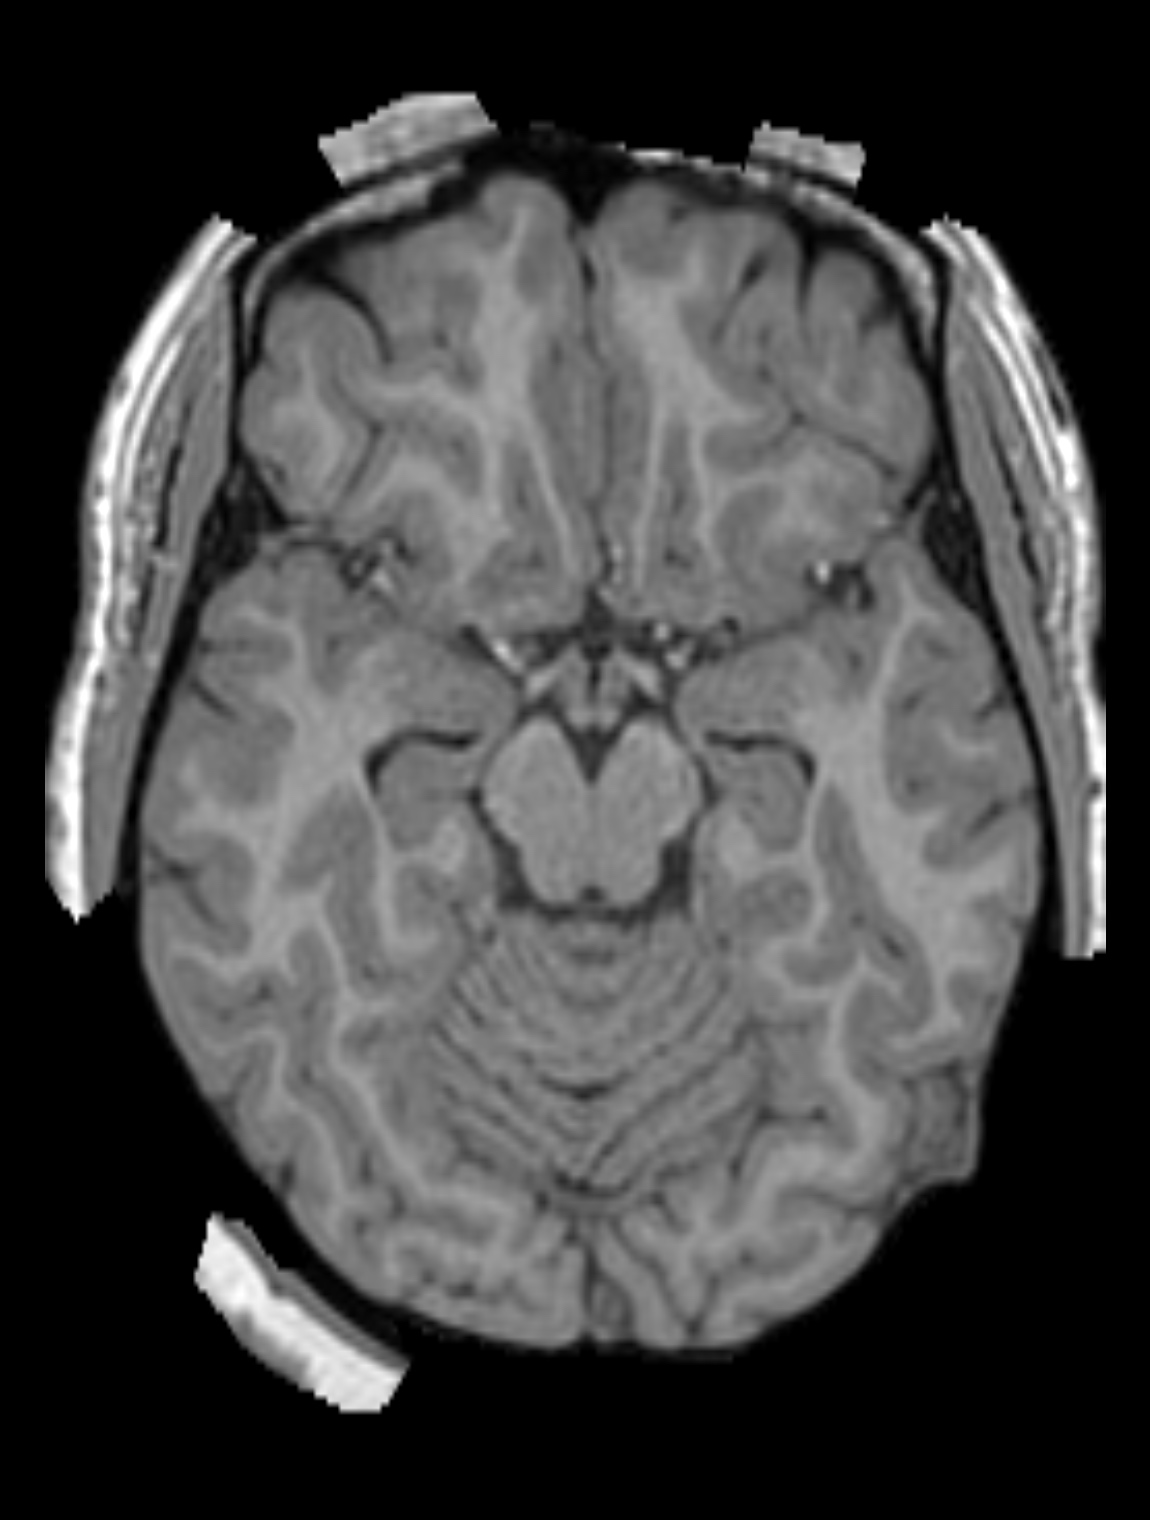
\includegraphics[scale=0.12]{img/Chap3/FSL54.jpg}
             \caption{Brain extracted with FSL}\label{fig:FSL54}
        \end{subfigure}
        \hfill
        \begin{subfigure}[b]{0.325\textwidth}
             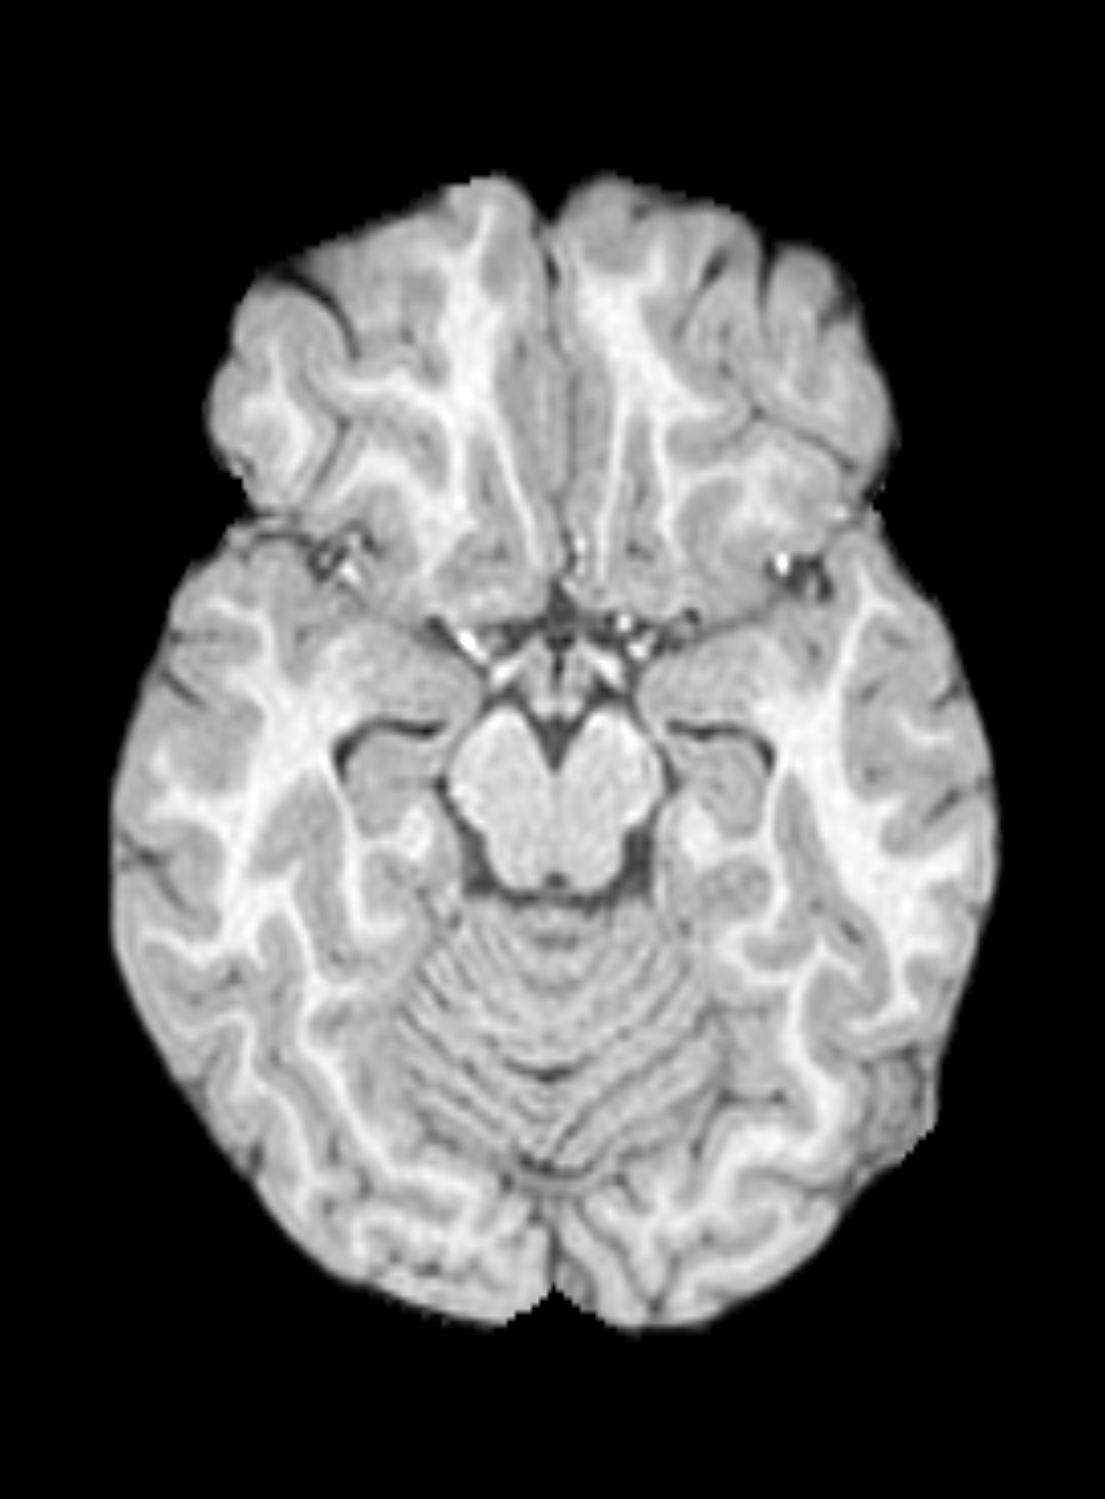
\includegraphics[scale=0.122]{img/Chap3/BRAIN54.jpg}
             \caption{Implemented pipeline}
        \end{subfigure}
        \caption{In the figure is reported the visual comparison of the brain extracted with FSL and the brain extracted with the proposed pipeline in two different cases. 
        The first row (Figures a, b, c) show a brain extraction that comparing the obtained brain mask with the one of FSL obtained a Dice coefficient of 0.95.
        The second row (images d, e, f) refers to a brain extraction that receive a Dice coefficient of $ 0.59$.}\label{fig:FSL_brain}
\end{figure}

The Dice coefficient is a metric to measure the overlapping between two images, then in the cases in which the FSL brain extraction is not the most desired one, as it is possible to see in the Figure \ref{fig:FSL54}, the measured metric could be low even when the implemented pipeline gives a correct result.

\paragraph{Tissue Segmentation:}
The tissue segmentation was evaluated mainly comparing the binary masks obtained by the proposed pipeline to the ones obtained by the FSL FAST algorithm, after a first evaluation by eyes, checking the eventually presence of visible errors.
In this way was found that on a minority of the volumes the algorithm used to merge two classes together, usually the white matter and the grey matter.
This kind of issue used to happen in images with a lower contrast as it is to see in \figureautorefname~\ref{fig:seg_fail}.
Looking at the probability maps obtained emerged that the lost class was correctly found but with a probability lower than the majority class (usually the white matter).

\begin{figure}[h!]
		\centering
        \begin{subfigure}[b]{0.49\textwidth}
             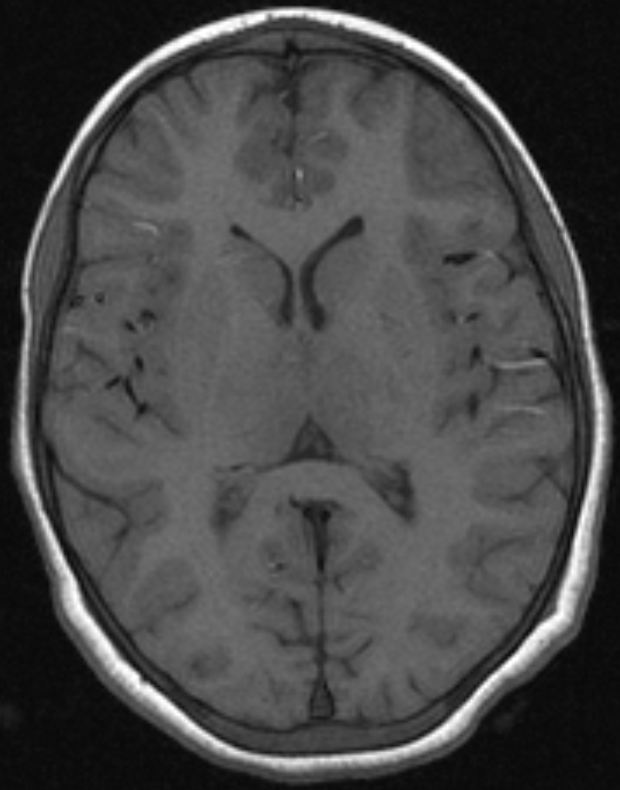
\includegraphics[scale=0.3]{img/Chap3/T1W0.png}
             \caption{Original Scan} 
        \end{subfigure}
        \hfill
        \begin{subfigure}[b]{0.49\textwidth}
             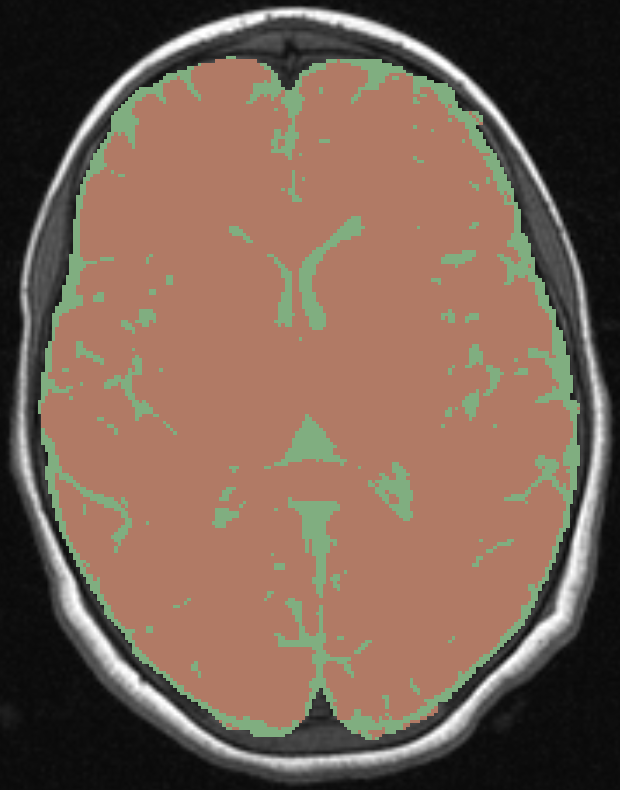
\includegraphics[scale=0.3]{img/Chap3/SEG0.png}
             \caption{Segmentation results}
        \end{subfigure}
        \caption{In Figure is reported a T1W scan and the result of a segmentation with the proposed algorithm. In this case is possible to observe how the low contrast of the original image lead to an erroneous segmentation in which the grey matter and the white matter are both classified in the same class (red) and only the cerebrospianl fluid is correctly classified (green). It is therefore important to say that the grey matter was correctly found in the partial volume maps but the associated probability was lower than the one in the white matter map.}\label{fig:seg_fail}
\end{figure}

Once the volumes were manually evaluated, a comparison between the masks obtained with FSL and the ones obtained with the proposed pipeline were computed measuring the obtained Dice coefficient.
For the images in which two classes were merged for the missing class was kept a Dice coefficient of $0$.
The obtained scores are reported in Table \ref{tab:segmentation_metrics}.

It is important to mention that the FSL algorithm failed in some cases as is possible to see in Figure \ref{fig:FSL_segmentation}.
This usually happened in those volumes where also the brain extraction failed.
Thus the Dice coefficient isn't a direct measure of the reliability of the proposed pipeline but an overlapping metric between the obtained masks and the masks computed by FSL, in the images in which FSL fails the obtained DSC is low even if the proposed pipeline manage to obtain a good segmentation. 

\begin{table}[h!]
\centering
\begin{tabular}{c|cccc}
                    & \textbf{Mean} & \textbf{Std. Dev.} & \textbf{Median} & \textbf{IQR} \\ \hline
\textbf{Brain Mask} & 0.87          & 0.12               & 0.93            & 0.11         \\
\textbf{WM}         & 0.78          & 0.19               & 0.83            & 0.19         \\
\textbf{GM}         & 0.67          & 0.30               & 0.80            & 0.28         \\
\textbf{CSF}        & 0.66          & 0.24               & 0.79            & 0.22        
\end{tabular}
\caption{In the table are reported the mean values, the standard deviation, the median value and the interquartile range of the Dice coefficient for the comparison between the binary masks for the brain, the white matter (WM), the grey matter (GM) and the cerebrospinal fluid (CSF) obtained with the proposed algorithm and the ones obtained with FSL BET (for the brain mask) and FAST (for the tissue segmentation).
As it is possible to see for the tissue segmentation the median is significantly higher than the mean.  This happened because the outliers of both the proposed pipeline segmentation (where two classes were merged) and the outliers of the FSL segmentation (in which the brain extraction failed, leading to a failing segmentation) were kept in account.}
\label{tab:segmentation_metrics}
\end{table}


\begin{figure}[H]
		\centering
        \begin{subfigure}[b]{0.325\textwidth}
             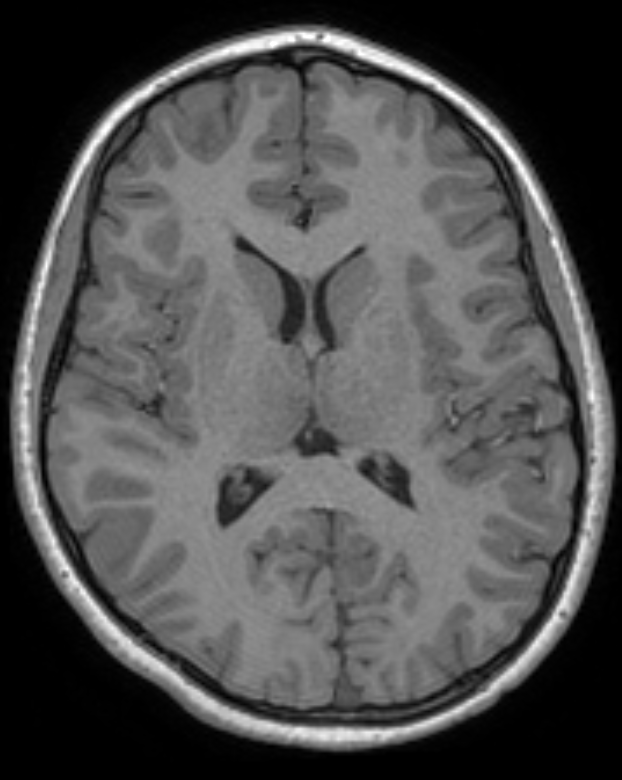
\includegraphics[scale=0.213]{img/Chap3/T1W48.png}
             \caption{Original scan}
        \end{subfigure}
        \hfill
        \begin{subfigure}[b]{0.325\textwidth}
             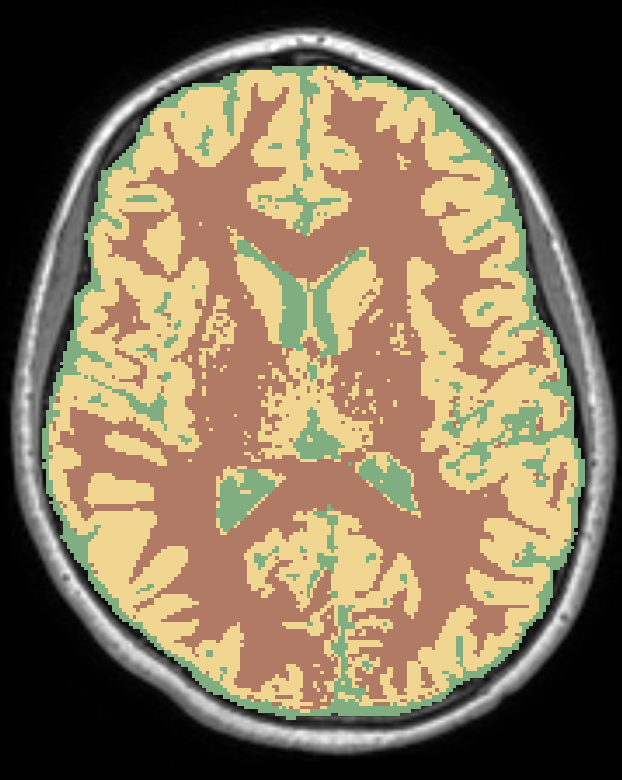
\includegraphics[scale=0.213]{img/Chap3/FSL_SEG48.png}
             \caption{FSL segmentation}
        \end{subfigure}
        \hfill
        \begin{subfigure}[b]{0.325\textwidth}
             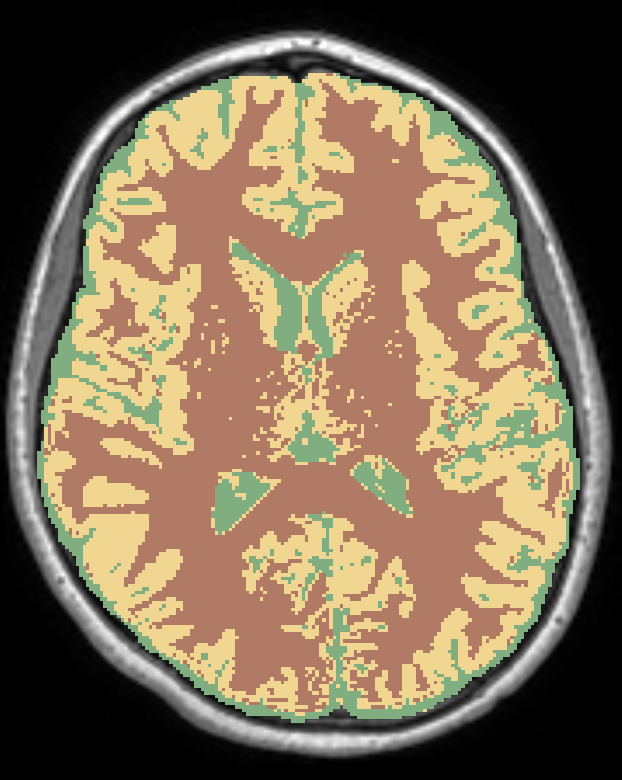
\includegraphics[scale=0.213]{img/Chap3/SEG48.png}
             \caption{Implemented pipeline}
        \end{subfigure}
        \hfill
        \begin{subfigure}[b]{0.325\textwidth}
             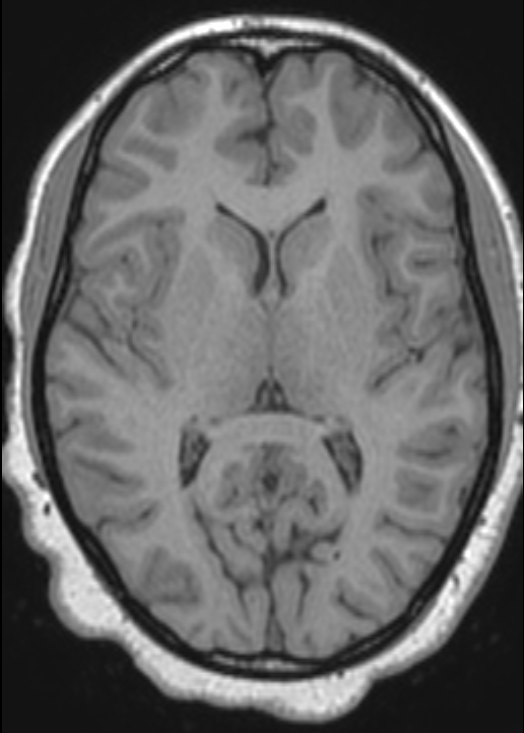
\includegraphics[scale=0.25]{img/Chap3/T1W54_2.png}
             \caption{Original scan}
        \end{subfigure}
        \hfill
        \begin{subfigure}[b]{0.325\textwidth}
             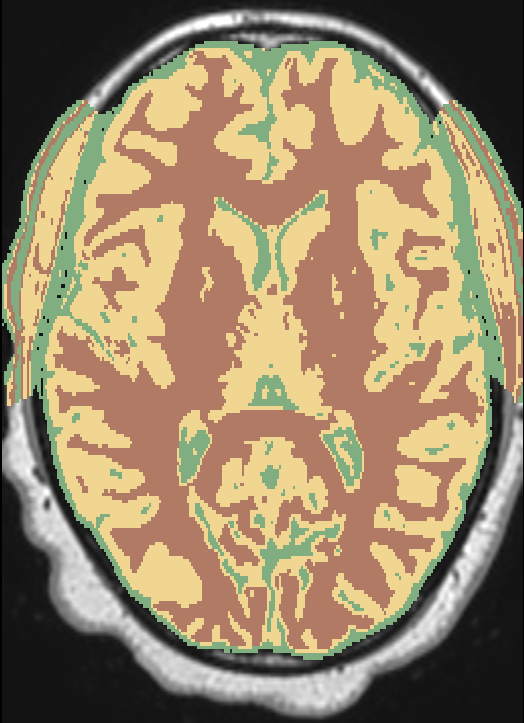
\includegraphics[scale=0.25]{img/Chap3/FSL_SEG54.png}
             \caption{FSL segmentation}
        \end{subfigure}
        \hfill
        \begin{subfigure}[b]{0.325\textwidth}
             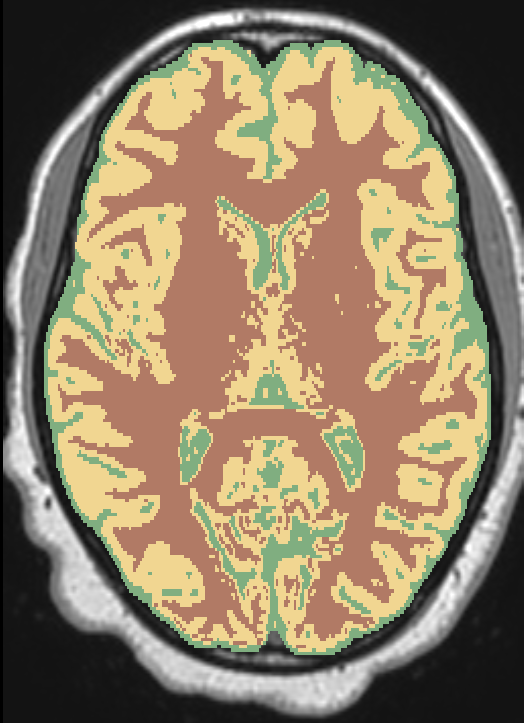
\includegraphics[scale=0.25]{img/Chap3/SEG54.png}
             \caption{Implemented pipeline}
        \end{subfigure}
        \caption{In the figure is reported the visual comparison of the brain segmented with FSL and the brain segmented with the proposed pipeline.
        The color scheme here used is red for white matter, yellow for grey matter and green for cerebrospinal fluid.
        The head scan for the second row (Figures d, e, f) is the same of Figure \ref{fig:FSL_brain} and in it is possible to see how a low quality segmentation lead not fully correct segmentation, concurring to obtain a lower Dice coefficient.}\label{fig:FSL_segmentation}
\end{figure}

On the images taken with an higher resolution it is possible to appreciate how the proposed pipeline correctly extract the brain and segment the image in its entire volume, as visible in \figureautorefname~\ref{fig:3Dseg}.

\begin{figure}[h!]
		\centering
        \begin{subfigure}[b]{0.325\textwidth}
             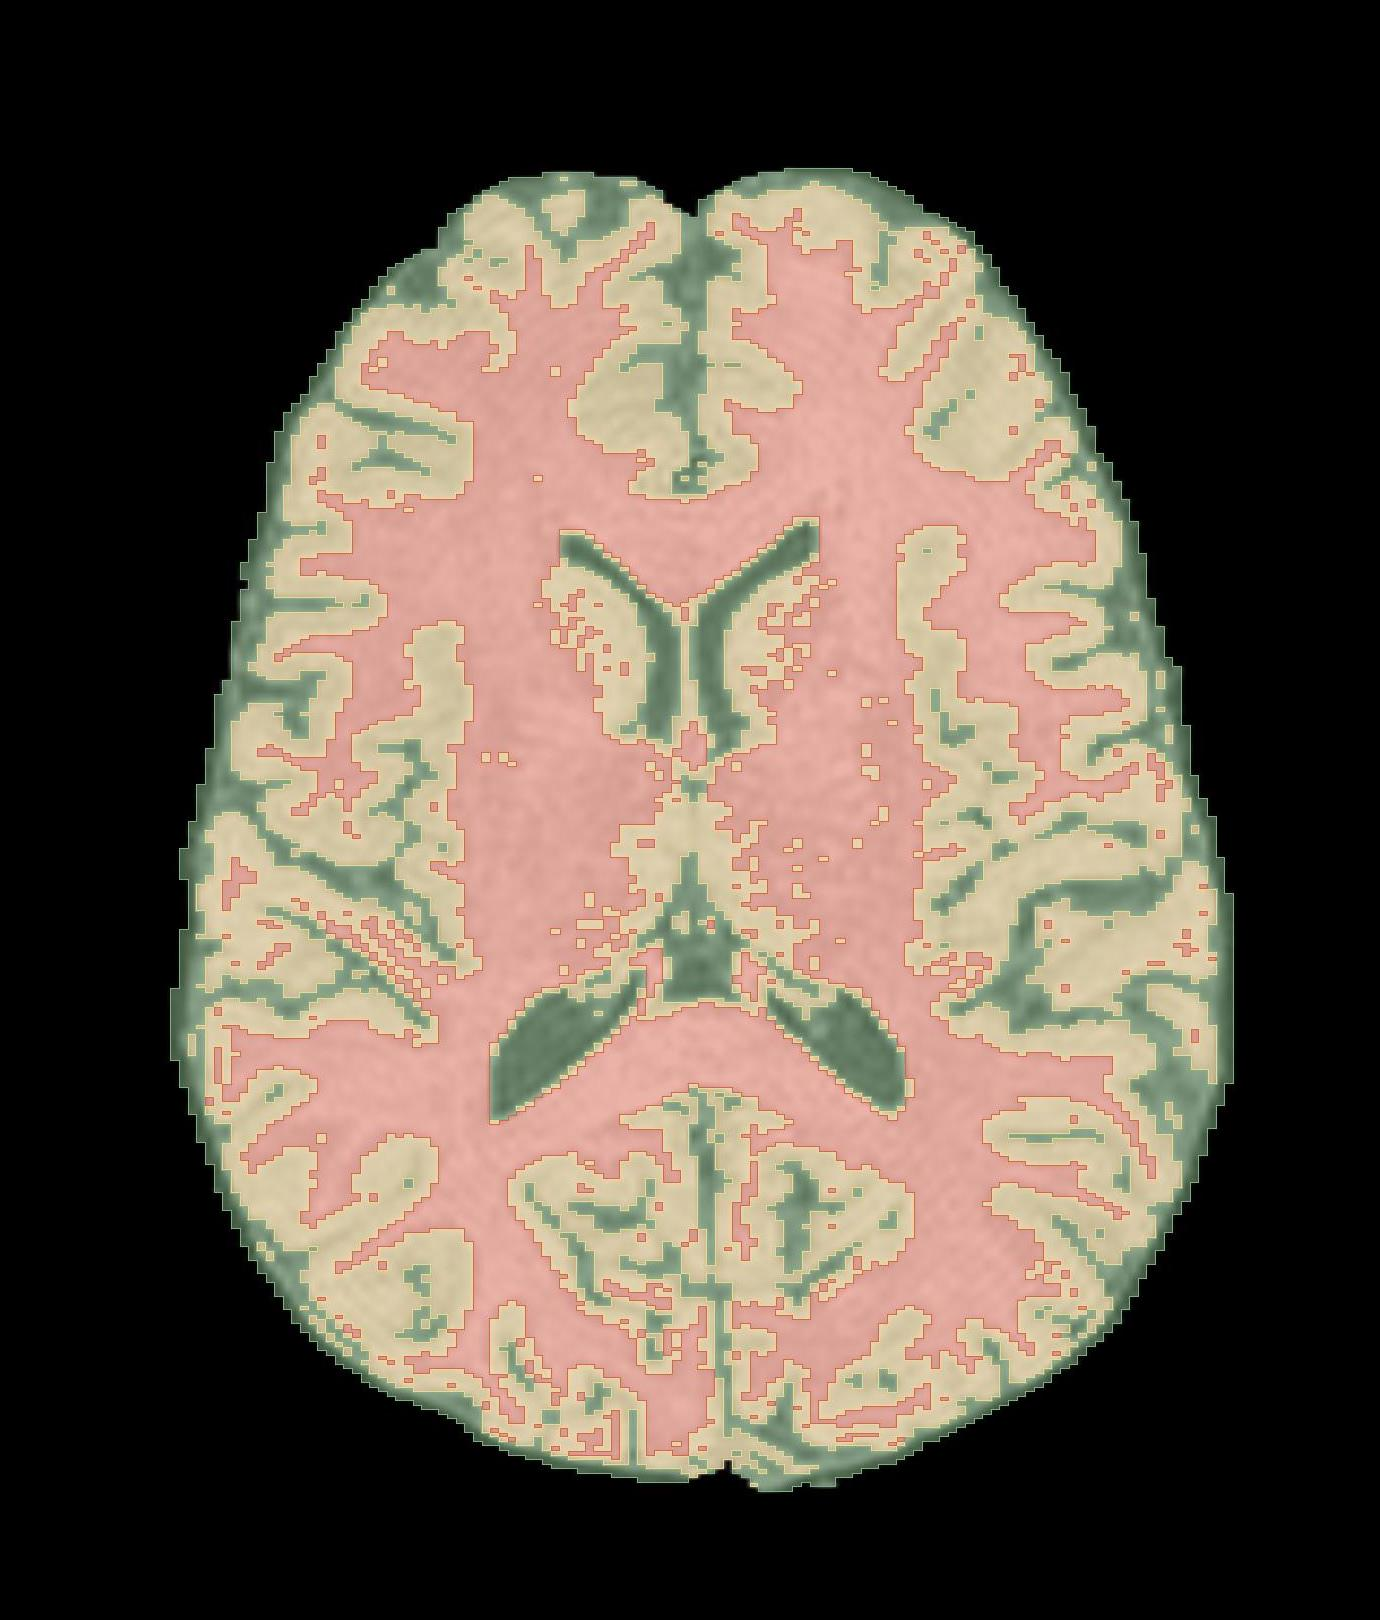
\includegraphics[scale=0.1046]{img/Chap2/segmented_axial.jpg}
             \caption{Axial view.}
        \end{subfigure}
        \hfill
        \begin{subfigure}[b]{0.325\textwidth}
             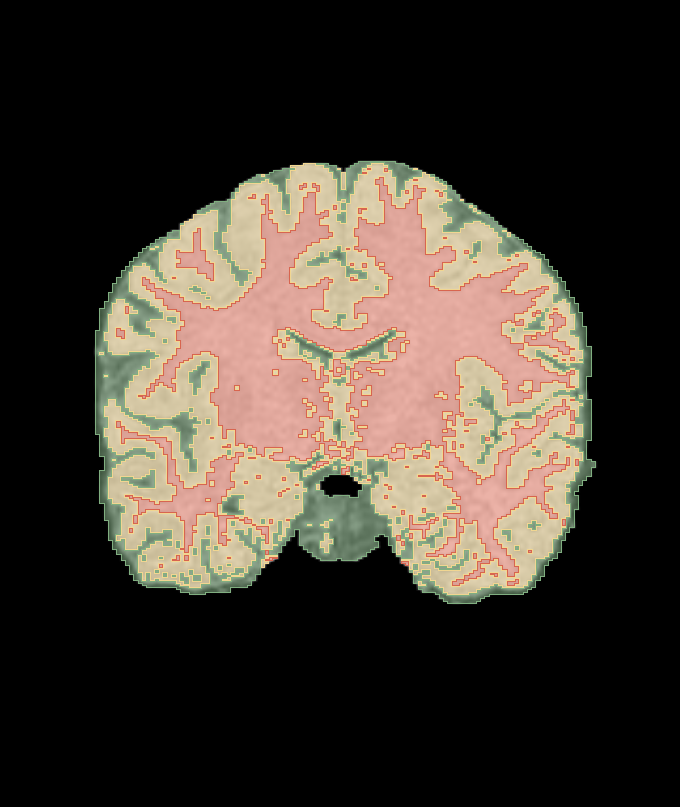
\includegraphics[scale=0.21]{img/Chap3/segmented_frontal.png}
             \caption{Frontal view.}
        \end{subfigure}
        \hfill
        \begin{subfigure}[b]{0.33\textwidth}
             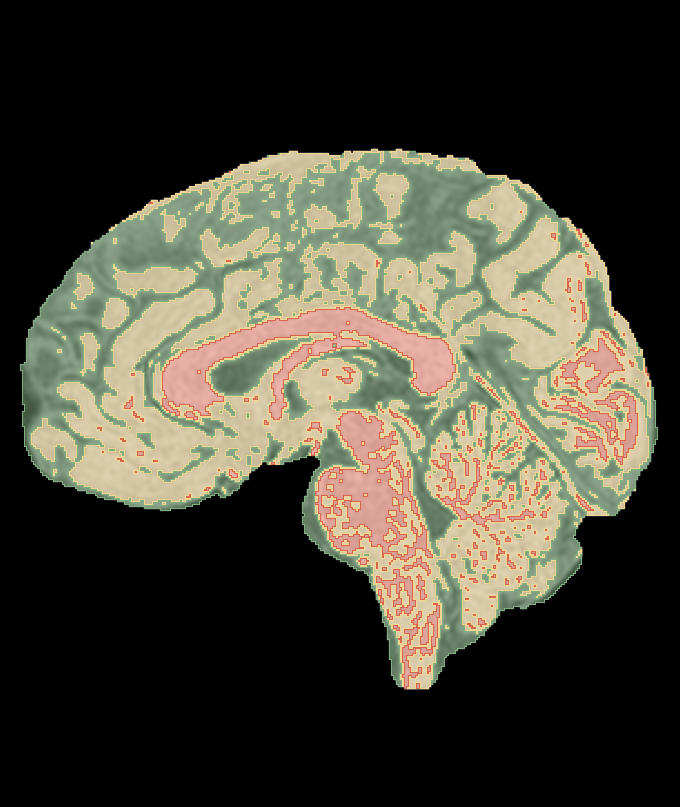
\includegraphics[scale=0.21]{img/Chap3/segmented_lateral.png}
             \caption{Lateral view.}
        \end{subfigure}
        \caption{3D visualization of the segmentation of an extracted brain. Looking at the three different points of view of the captured volume (axial view, frontal view and lateral view) is possible to appreciate how the full brain volume was extracted from the unwanted head structures and  segmented in white matter (red), grey matter (yellow) and cerebrospinal fluid (green).} \label{fig:3Dseg}
        \end{figure}


\section{Post-Processing}

The provided data set was divided in two subsets. The first one is comprehensive of $51$ images, in which the U-Net ensemble found a total of $5581$ lesions, and constitute the \textit{training set}, used to train the chosen classifiers.
The remaining $6$ images containing $425$ total labels of which $99$ are considered true, constitute an independent \textit{test set}, used to evaluate the classification performances.

The goodness of the classifiers was evaluated comparing the labels classified by the three proposed approach with the ones classified "a priori", measuring the modified Jaccard score for overlapping with the manual segmentation, as shown in equation \ref{eq:modified_jaccard}.
To have a quantitative comparison were used different metrics in order to take in account of all the possible difference between the three implemented classifiers. The results, for each classifiers are reported in Table \ref{tab:postprocessing_metrics}.
The first researched characteristic for the three classifiers was to have an high recall value, in order to be more conservative toward the lesions correctly found by the U-Net ensemble. This characteristic was satisfied by all the implemented classifier.
The classifier which gained the highest values for all the metrics was the random forest classifier, which however is the less explainable one. For this reason also the other two classifiers were kept during the work of thesis.
It is interesting to compare the decision tree and the logistic regression because, even if the decision tree classifier have greater balance accuracy and recall, the logistic regression classifier gains an higher AUC ROC score and especially an higher AUC precision-recall score, a metric that is particularly suited for unbalanced data \cite{ART:AUCPR}.
It is important to compare the result obtained for the area under precision-recall curve with the ones that a random classifier would have gained with the proposed set of data: since the data are unbalanced with a positives ratio of about $0.23$ the expected score for a random classifier is of $0.23$.

\begin{table}[h!]
\small
\begin{tabular}{c|ccccc}
 & \textbf{Bal. Acc.} & \textbf{AUC ROC} & \textbf{AUC PR} & \textbf{Precision} & \textbf{Recall} \\ \hline
\textbf{Decision Tree}       & 0.74 & 0.81 & 0.45 & 0.38 & 0.96 \\
\textbf{Logistic regression} & 0.68 & 0.83 & 0.61 & 0.32 & 0.96 \\
\textbf{Random Forest}       & \textbf{0.74} & \textbf{0.90} & \textbf{0.74} & \textbf{0.38} & \textbf{0.97}
\end{tabular}
\caption{In the table are reported the results of the five evaluated metrics (balanced accuracy, area under ROC curve, area under precision-recall curve, precision and recall) comparing the classified labels with the ones 'a priori' classified for all the three implemented classifiers (decision tree, logistic regression and random forest).
As it is possible to appreciate all the classifiers obtain a very high value for the recall, which means that very few classified data are found to be \emph{false negative}.
The Random Forest classifier obtains the higher value in all the remaining metrics and therefore is the one that also classify correctly the greatest number of negative lesions.}
\label{tab:postprocessing_metrics}
\end{table}

In the end was also interesting to look at the importance of the features for the decision tree and the random forest classifiers and to look at the coefficient given at each feature by the logistic regression. This gave us important informations about the functionality of the U-Net ensemble. The results obtained are reported in Table \ref{tab:feature_importance}.
It was discovered that both the random forest classifier and the decision tree didn't took in account at all for the probability given as output from the U-Net ensemble and the logistic regression gave it a strong negative value.
As a check this feature was removed from all the classifier and the results obtained for the measures of the different metrics evaluated didn't change significantly. 
Another interesting discovery was the high relevance given to the white matter probability map, meaning that the U-Net ensemble have the tendency to find lesions also outside the white matter, probably due to the working characteristic of the U-Net to consider one slice per time, and then suffer the possible partial volume effect.


\begin{table}[h!]
\centering
\small
\setlength\tabcolsep{1pt}
\begin{tabular}{c|ccccccc}
                & \textbf{Prob.}     & \textbf{Size}        & \textbf{Boundary}     & \textbf{Exclusion} & \textbf{WM}       & \textbf{GM}        & \textbf{CSF}       \\ \hline
\textbf{Dec. Tree} & 0.000 & 0.0133 & 0.032 & 0.034 & 0.659 & 0.042 & 0.098 \\
\textbf{Log. reg.} & 0.00 & $8.83 \times 10^{-2}$ & 0.236 & -1.50 & $1.07 \times 10^5 $ & $4.58 \times 10^4$ & $7.82 \times 10^3$ \\
\textbf{Rnd F.} & $0.000$ & $0.146$ & $0.027$ & $0.029$  & $0.615$ & $0.067$ & $0.116$
\end{tabular}
\caption{Table reporting the importance of the features for the decision tree and random forest classifiers. 
The features indicated are the probability in output from the U-Net, the physical size of the lesion, the overlapping with a manually defined boundary and exclusion regions and the probability to be in the white matter, grey matter or cerebrospinal fluid.
For the logistic regression classifier the coefficients associated at the features are reported. It can be seen how the classifiers take in account the different features and for example evaluating which feature can be removed.}
\label{tab:feature_importance}
\end{table}


\end{document}